\title{AWS Academy}
\author{Richard Thomas}
\date{\week{1}}

\maketitle

\section{Introduction}
In this course we use AWS Academy as a resource to learn how to deploy and manage infrastructure on Amazon Web Services (AWS),
as an example of a cloud based Infrastructure as a Service (IaaS) and Platform as a Service (PaaS) environment.
You have been enrolled in three AWS Academy courses, as well as the AWS Learner Lab.
We expect you to work your way through at least two of the AWS Academy courses as self-study material.
The \link{CSSE6400 course schedule}{https://csse6400.uqcloud.net/schedule/} provides a guide as to when we expect you to complete particular modules in the
\link{AWS Academy Cloud Foundations}{https://awsacademy.instructure.com/courses/73523},
and \link{AWS Academy Cloud Architecting}{https://awsacademy.instructure.com/courses/73526} courses.

The \link{AWS Academy Cloud Developing}{https://awsacademy.instructure.com/courses/73525} course is provided as a supplementary resource.
It covers much of the same content as \link{AWS Academy Cloud Architecting}{https://awsacademy.instructure.com/courses/73526}, 
but \link{AWS Academy Cloud Architecting}{https://awsacademy.instructure.com/courses/73526} does so in a more structured and progressive manner.
\link{AWS Academy Cloud Developing}{https://awsacademy.instructure.com/courses/73525} treats each topic a little more independently.
The advantage of this is that it also covers a couple of other topics, such as REST APIs and Containers, that you may find useful.

\link{AWS Academy Learner Lab}{https://awsacademy.instructure.com/courses/73527} will be used in practical sessions from week 4 onwards.
You will also use it to implement your solution to the Cloud Infrastructure assignment.

You need to accept your enrolment into:
\begin{itemize}
    \item AWS Academy Cloud Foundations [\href{https://awsacademy.instructure.com/courses/73523}{73523}] course;
    \item AWS Academy Cloud Architecting [\href{https://awsacademy.instructure.com/courses/73526}{73526}] course;
    \item AWS Academy Cloud Developing [\href{https://awsacademy.instructure.com/courses/73525}{73525}] course; and
    \item AWS Academy Learner Lab [\href{https://awsacademy.instructure.com/courses/73527}{73527}] course.
\end{itemize}
And then login to the AWS Academy and navigate to your courses.

\section{AWS Academy}
AWS Academy is an educational platform to teach you how to use AWS services.
The content has been created by key developers in the AWS team.

\subsection{Enrol in AWS Academy}

\begin{enumerate}
    \item
        Set up your AWS Academy account by responding to your email invitation and clicking \textbf{Get Started}.
        The email invitation will come from AWS Academy.
        Check your junk/spam folders.

        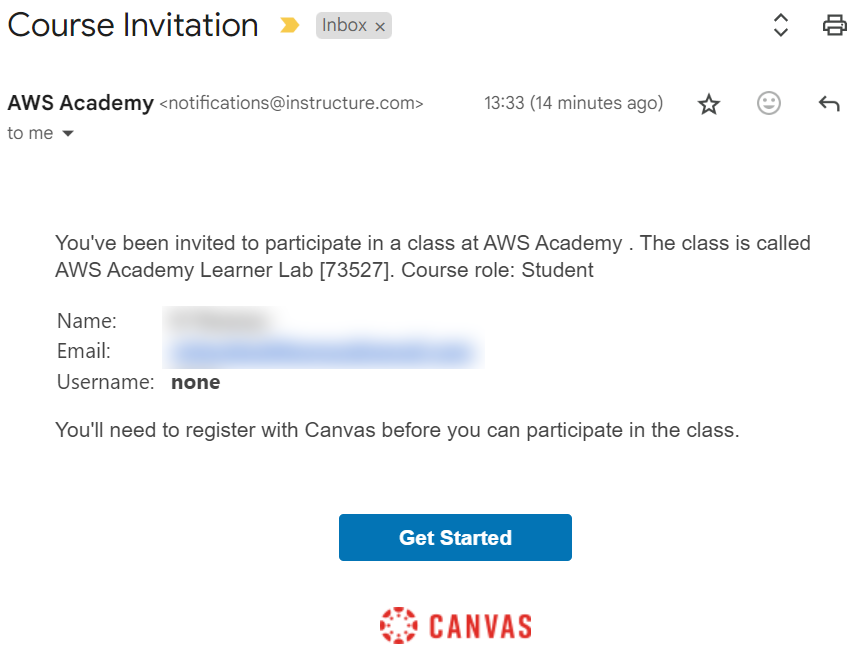
\includegraphics[width=0.8\textwidth]{images/email-invite}

    \item Go to \url{https://www.awsacademy.com/vforcesite/LMS_Login} to login.
    \begin{enumerate}
        \item Press \textbf{Student Login}.
        \item Use the email address that received the email invitation.
    \end{enumerate}

    \hspace{9mm}
    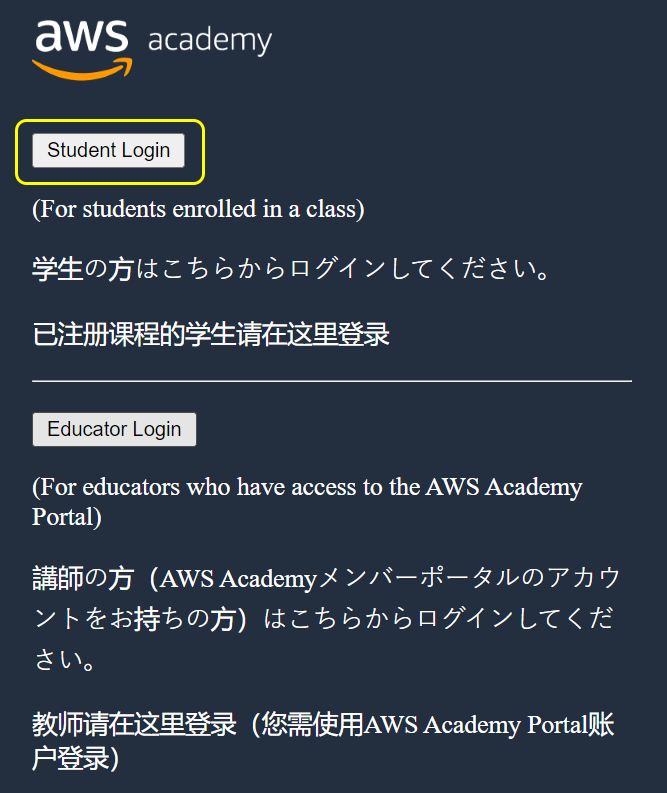
\includegraphics[height=0.35\textheight]{images/labs-login1}
    \hspace{5mm}
    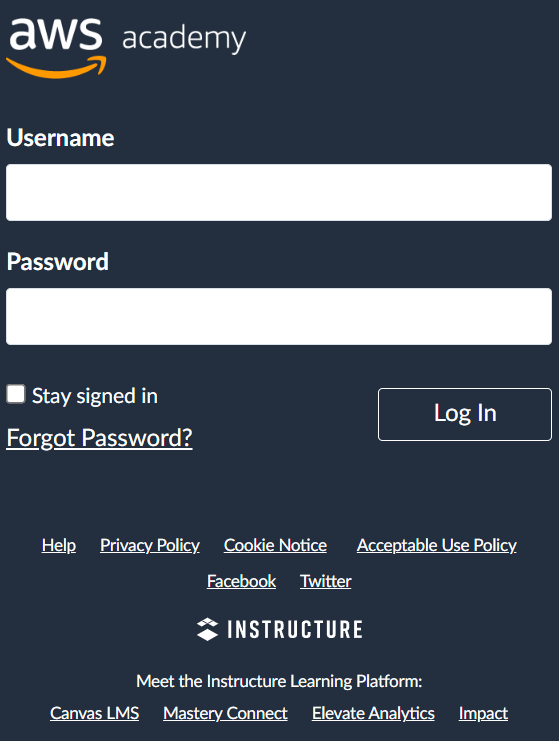
\includegraphics[height=0.35\textheight]{images/labs-login2}
\end{enumerate}


\subsection{Exploring the Interface}
Once you login, you should see your account dashboard.
This lists the courses in which you are enrolled.

\vspace{4mm}
\noindent
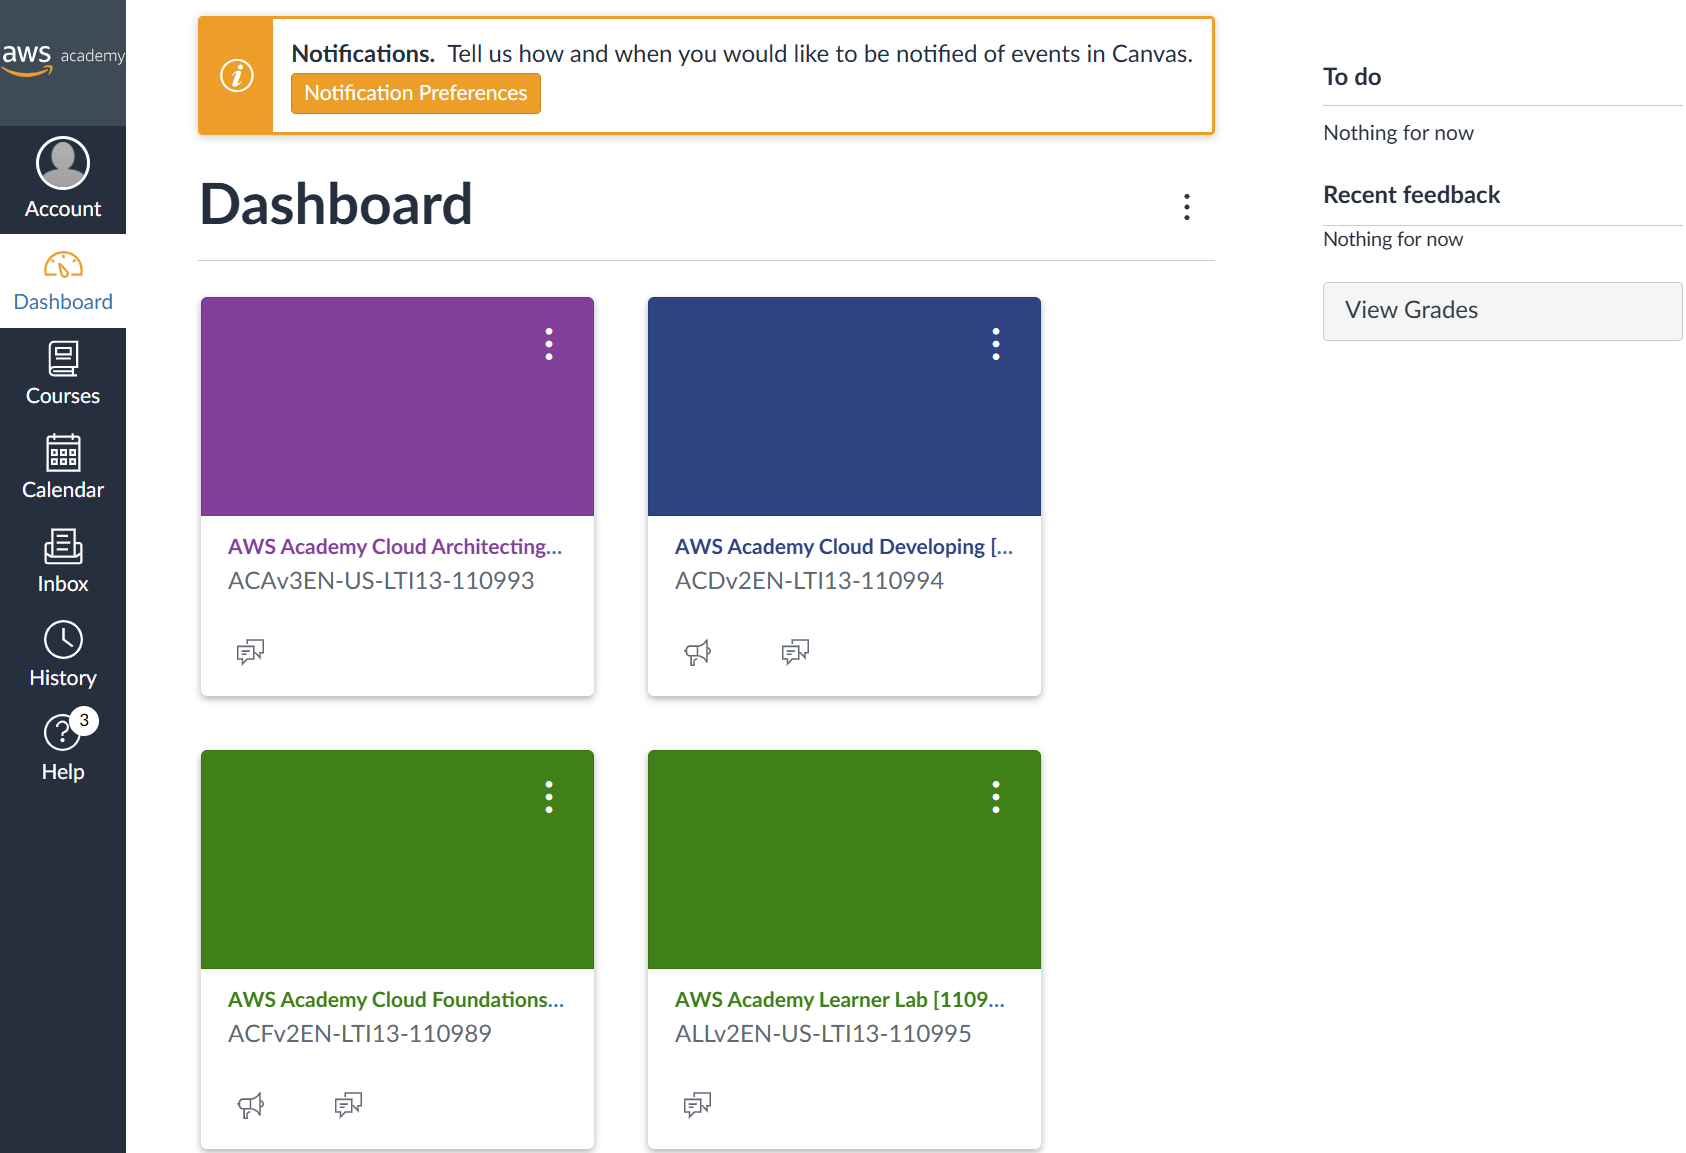
\includegraphics[width=\textwidth]{images/dashboard}
\vspace{2mm}

\noindent
Click on a course to go to its home page.

\vspace{4mm}
\noindent
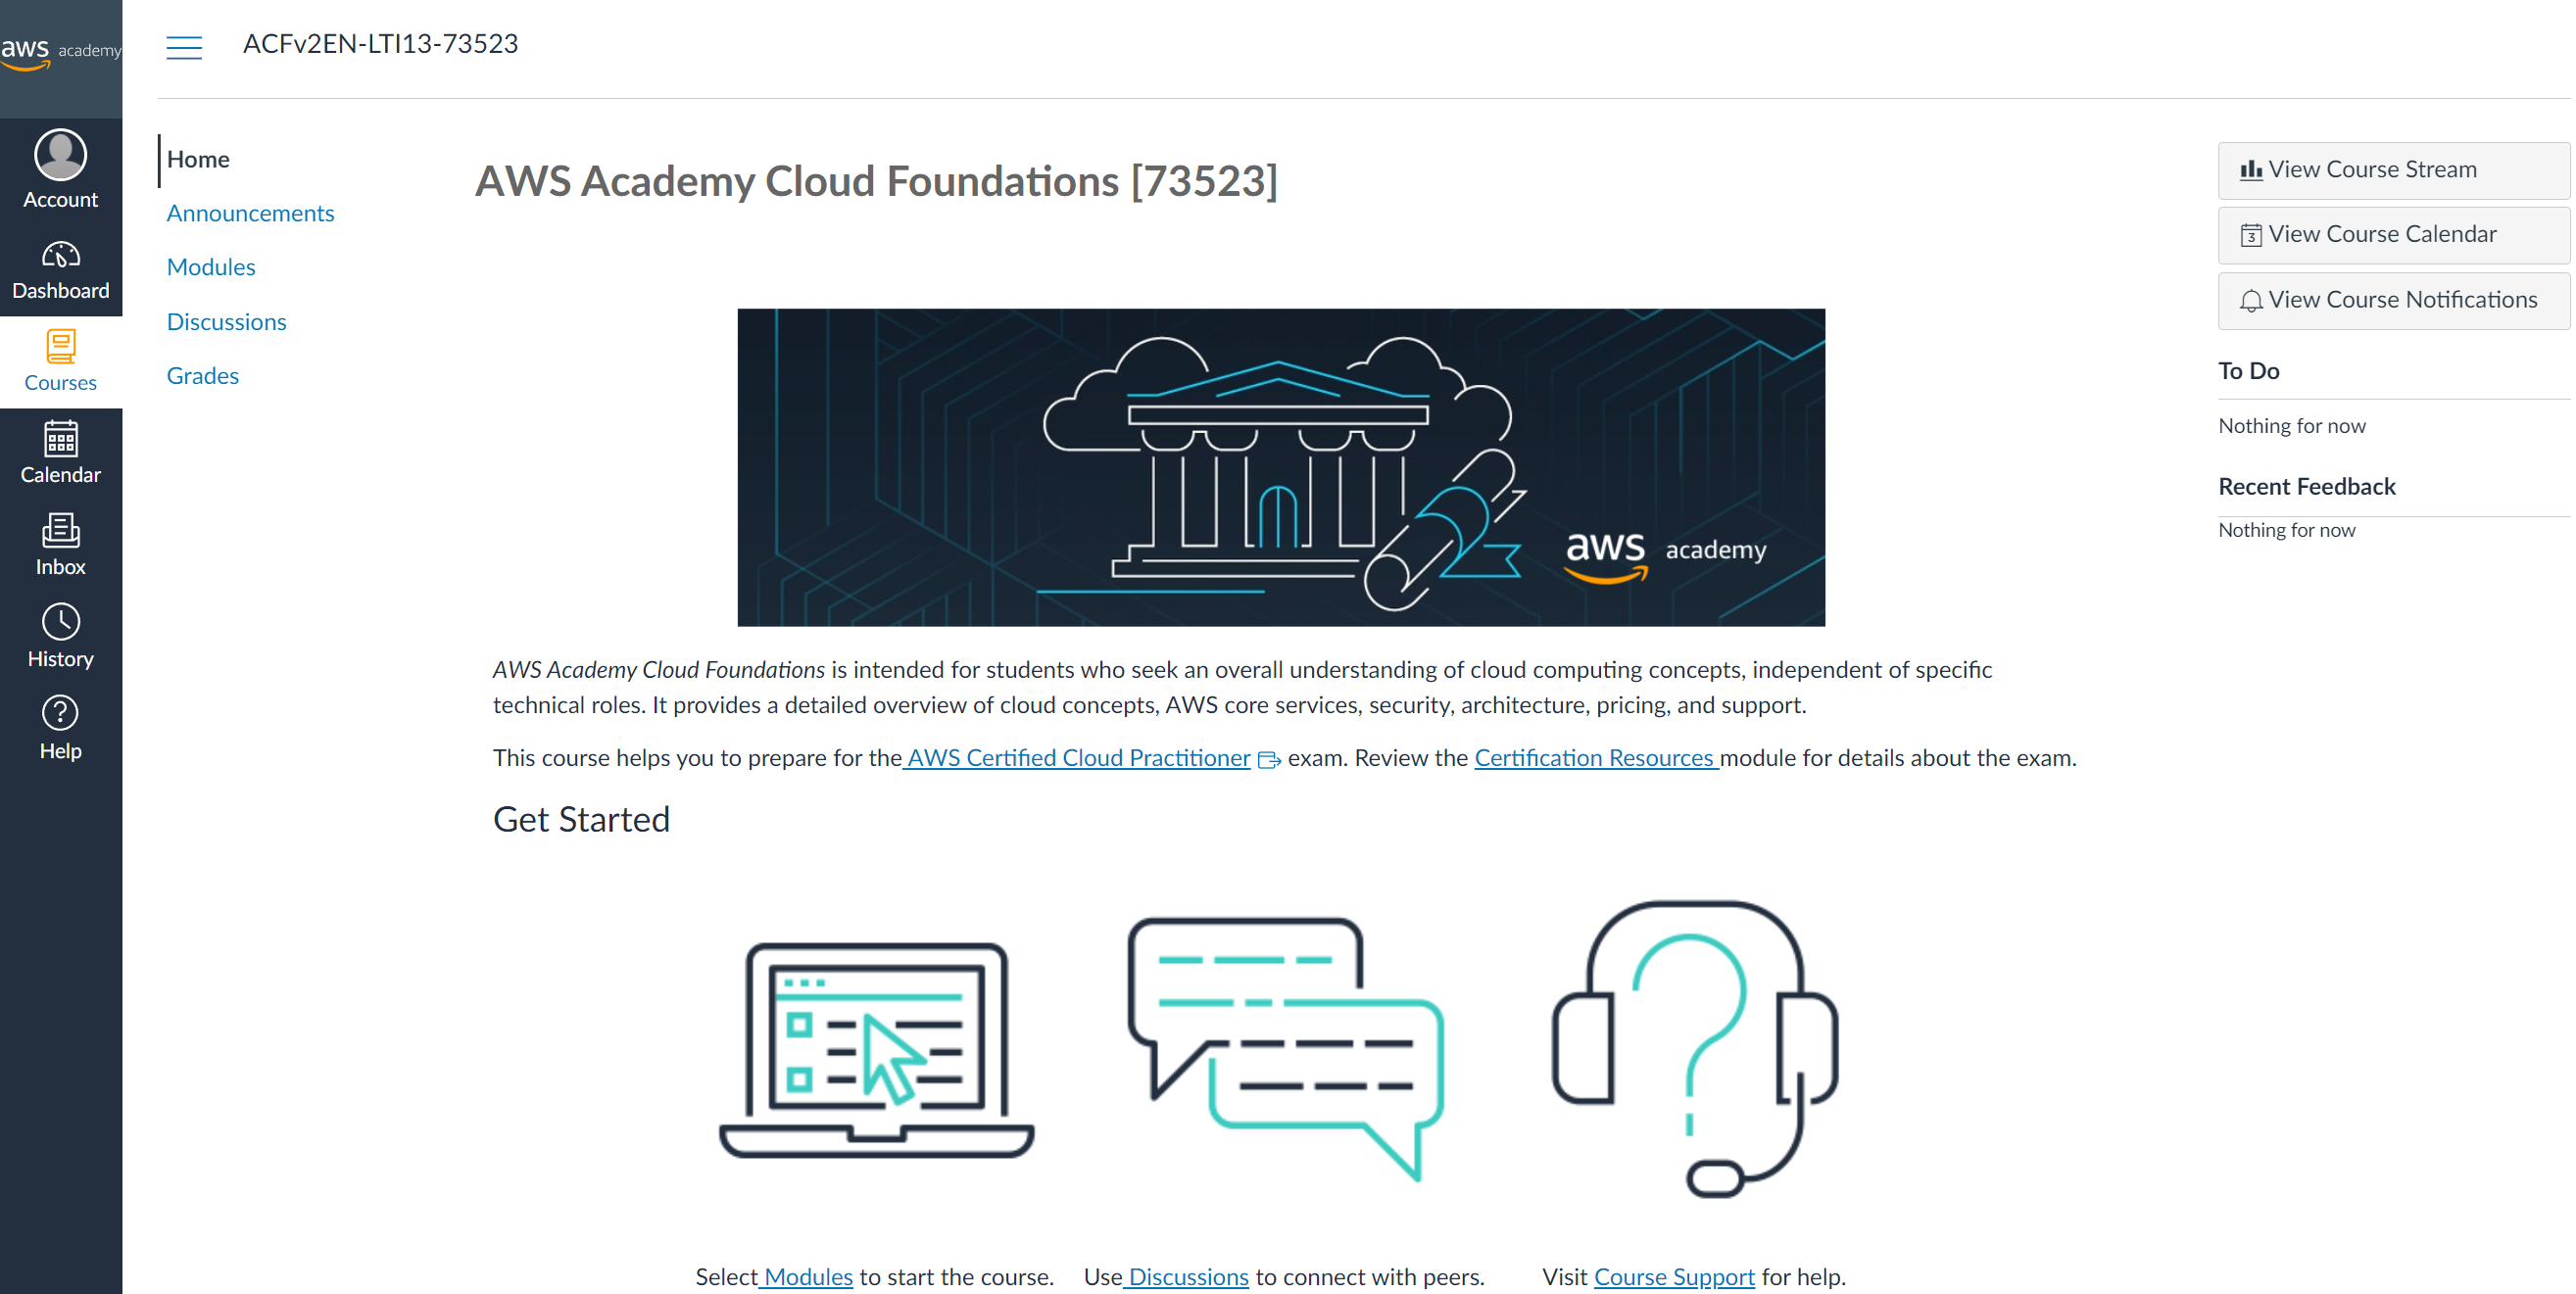
\includegraphics[width=\textwidth]{images/foundations-home}
\vspace{3mm}

\noindent
Navigate to the \texttt{Modules} tab and you will see the list of modules and their learning content for the course.
The content includes videos, readings, and self-assessment exercises.
The self-assessment exercises are to help you to know that you understand the content.
These are not used as part of your assessment in this course.

\vspace{4mm}
\noindent
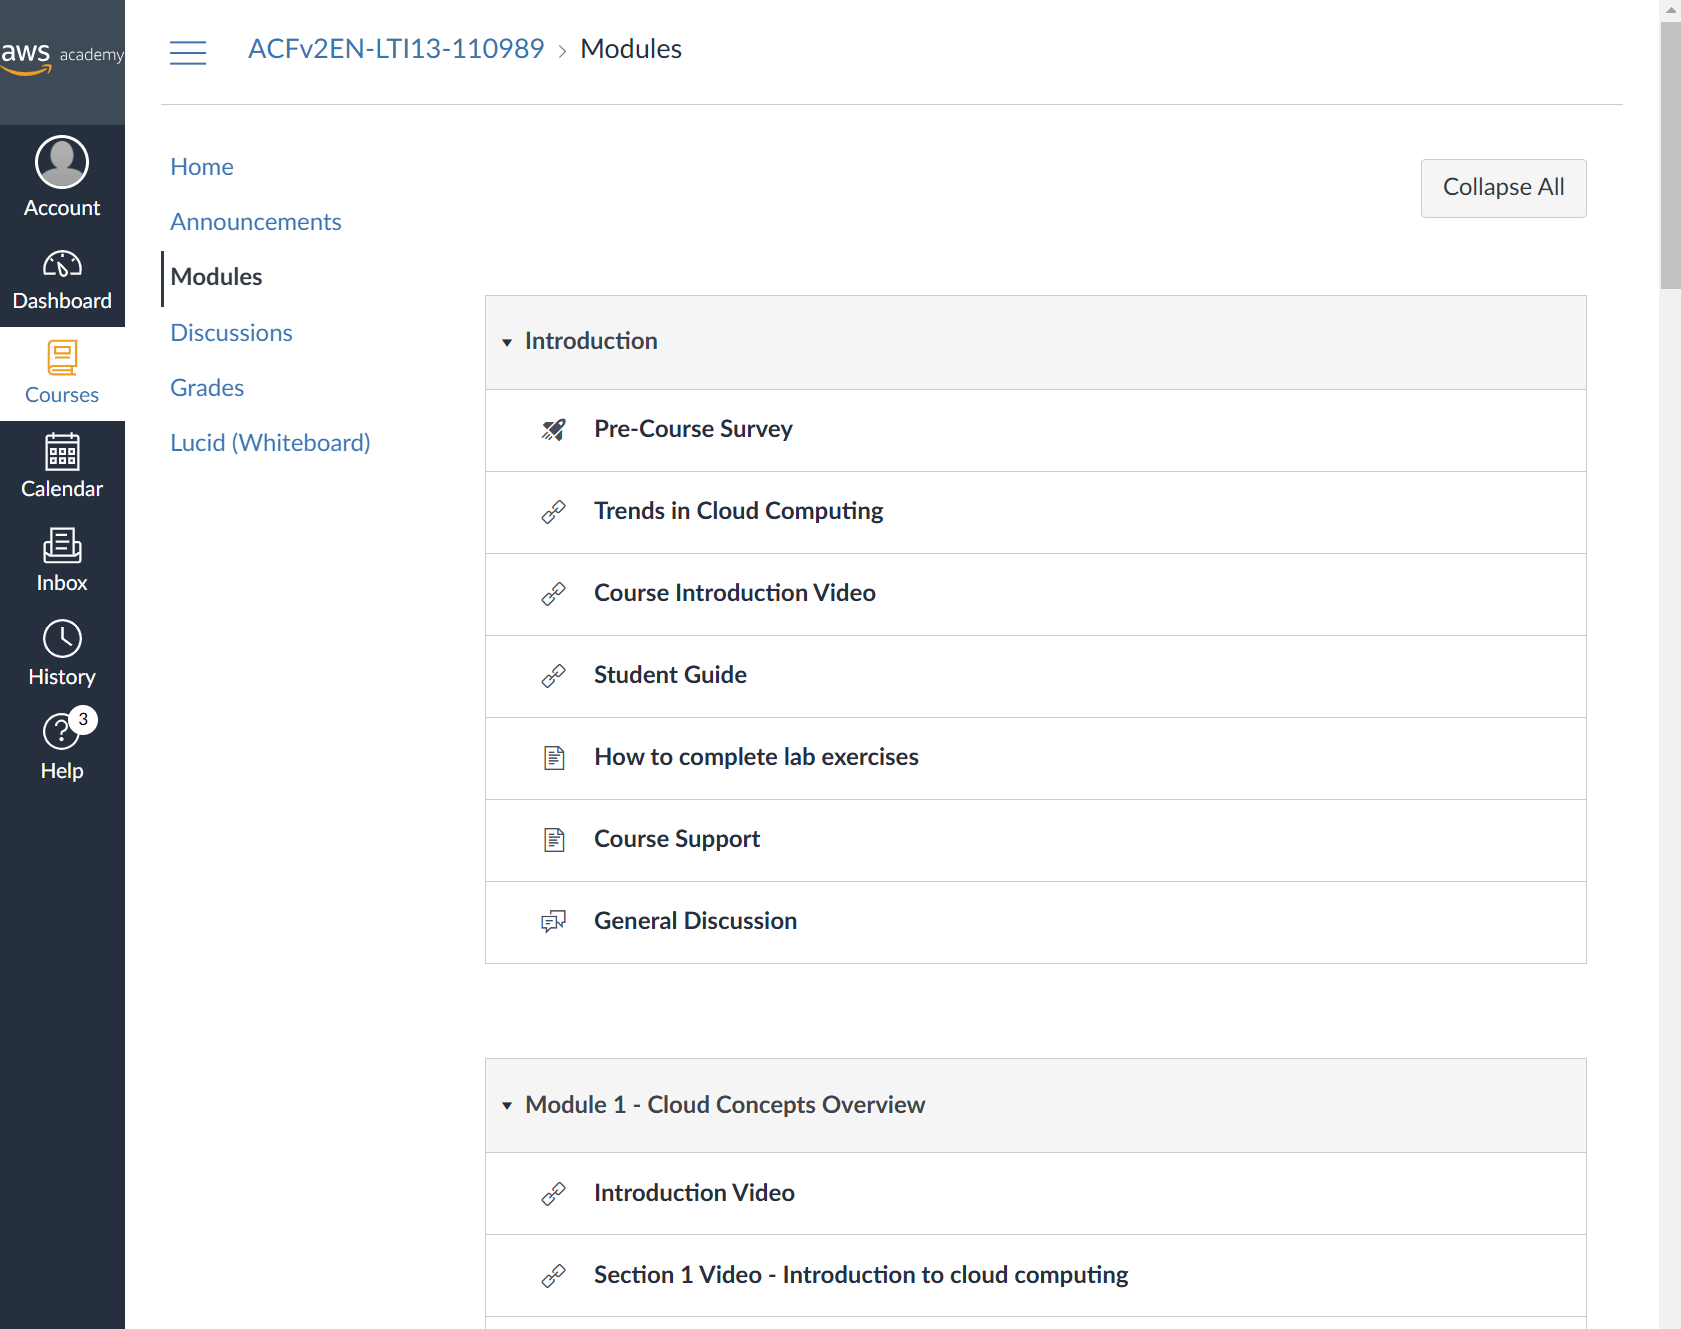
\includegraphics[width=\textwidth]{images/modules}
\vspace{2mm}

\noindent
Explore the AWS Academy interface and courses.
Start working through the \link{AWS Academy Cloud Foundations}{https://awsacademy.instructure.com/courses/73523} course.
Try to complete at least half of it this week.
